\section{Action Path Models}
\label{ch:model}

\epigraph{It is impossible to separate a cube into two cubes, or a fourth power into two fourth powers, or in general, any power higher than the second, into two like powers. I have discovered a truly marvelous proof of this, which this margin is too narrow to contain.}{Pierre de Fermat}

In this chapter, we formalize few concepts and metrics in clickstream data,
and then describe a proposed clickstream model named \emph{Action Path model} 
based on recurrent nerual network that models a client side web browsing behavior. 
An \emph{action path} is different than the original clickstream concept since 
a user may \emph{switch browser tabs} for parallel viewing \cite{huang2010parallel} or uses \emph{back button} 
for backtracking viewing \cite{huang2012no} as we discussed in Chapter \ref{ch:relate}, 
namely, a user performes a visit action.
A server side collected clickstream does not containing such detailed level of 
user clickstream.
The term \emph{action path} is a generalized concept of clickstream, 
which replaces individual URLs to chronological ordered user actions 
(with backbutton and browser tab switch effects) in a browser.
Figure \ref{fig:clickstream} illustrates a simplified version of an action path that 
compares vanilla clickstream.

\begin{figure}[H]
    \centering
    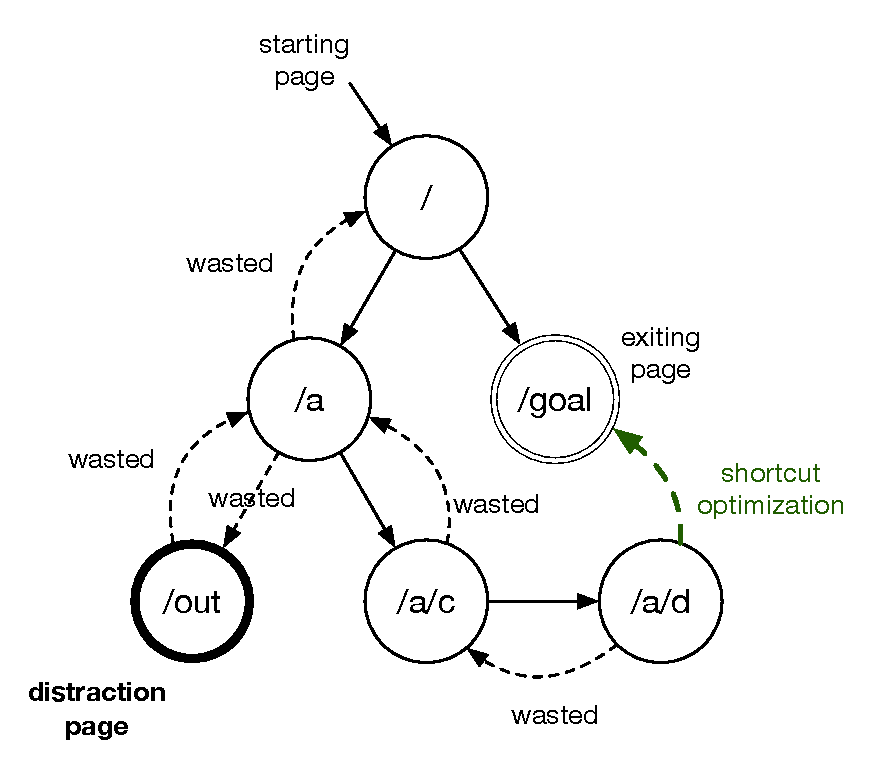
\includegraphics[width=0.5\textwidth]{figures/clickstream}
    \caption{A simple action path. A user starts from the starting page, and performed
    a series of page click actions, ends on a exiting page. 
    The server side records clickstream in the following order:
    / $\rightarrow$ /a $\rightarrow$ /out $\rightarrow$ /a/c $\rightarrow$ /a/d $\rightarrow$ /goal.
    However the actual user actions are: 
    / $\rightarrow$ /a $\rightarrow$ /out $\rightarrow$ /a $\rightarrow$ /a/c $\rightarrow$ /a/d 
    $\rightarrow$ /a/c $\rightarrow$ /a $\rightarrow$ / $\rightarrow$ /goal. 
    The records from server side lost the interaction details between users and browsers.
    Node that /out is a distraction page in the graph, 
    which may located in a different website (e.g. advertisement), 
    and black dashed arrorws are wasted user
    actions. The /goal page may not clear in the beginning of the clickstream, one can generate
    a shortcut optimization navigation to the /goal page while more clickstream context
    be presented, i.e. an optimized user action is 
    / $\rightarrow$ /a $\rightarrow$ /a/c $\rightarrow$ /a/d $\rightarrow$ /goal. In this case,
    the demand page of the visit session is discovered in /a/d.}
    \label{fig:clickstream}
\end{figure}

For a convinience of discussion, \textbf{we indiscriminate the use of 
term \emph{action path} and \emph{clickstream} in
this thesis to indicate a chronological ordered user actions}.

\subsection{Completion Effeciency}

An action path of a visiting session starts from a starting page and ends on a exiting page.
Since we consider the effect of browser back button and browser tab swtichs, 
a previous page could easily be visited twice, if a user clicked the back button. 
Therefore, a page may directs to multiple pages. 
\emph{For instance, an action path can degrade to a linked list if the user
click through different pages without using back button and switching tabs; or an action
path can become a 1-to-n bipartite graph if a user use back button back to previous page
after clicked a page or only switching tabs from a specific page to one another}, 
as shown in Figure \ref{fig:sim-action-path}.

As a result, we define a term \emph{completion effeciency} based on shortest path from starting page
to exiting page, and stay duration of the action path. 

\begin{figure}[H]
    \centering

\begin{subfigure}[b]{0.55\textwidth}
    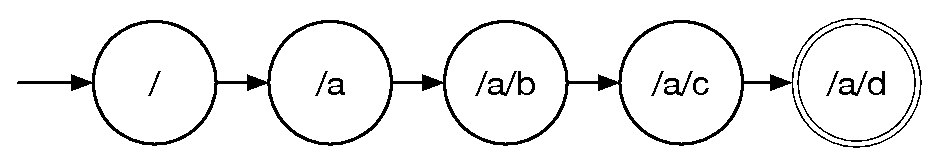
\includegraphics[width=1\textwidth]{figures/linked-list}
    \caption{}
    \label{fig:sim-action-1}
\end{subfigure}
    
\begin{subfigure}[b]{0.23\textwidth}
    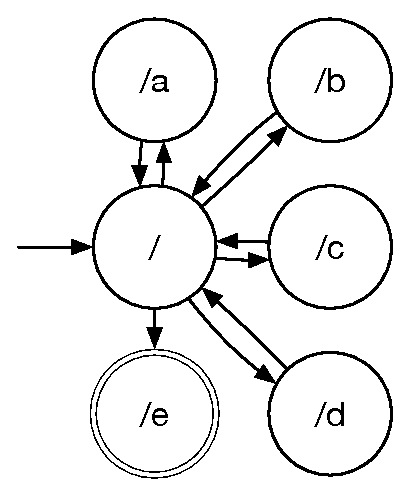
\includegraphics[width=1\textwidth]{figures/1ton}
    \caption{}
    \label{fig:sim-action-2}
\end{subfigure}

\caption{Two special case of an action path: an action path that degrade to a linked list if the user
click through different pages without using back button and switching tabs (\ref{fig:sim-action-1}), and 
an action path that represented in 1-to-n bipartite graph if a user use back button back to previous page
after clicked a page or only switching tabs from a specific page to one another (\ref{fig:sim-action-2}).}
\label{fig:sim-action-path}
\end{figure}

Let an action path is represented by a directed cyclic graph, each node represents a visited page,
and each edge has a weight that represents the stady duration of its tail node.
Assume the total stay duration of the shortest path from starting page to existing page
is $d_s$, and the total stay duration of the action path is $D$, 
the number of nodes in the shortest path is $n_s$, the total nodes 
in an action path is $N$, we define the \emph{completion effeciency $E$} is 
as follows Equation \ref{eqn:completion-effeciency}:

\begin{align}
\label{eqn:completion-effeciency}
\begin{split}
    E = w_1 \frac{n_s}{N} + w_2 \frac{d_s}{D}\\
    w_1 + w_2 = 1
\end{split}
\end{align}

where $w_1$, $w_2$ are hyperparameters to balancing the importance of action path 
and stay duration. According to the discussion of two special case of action path,
it is trivial to show the range of $E$ is $(0, 1]$. As a complement, we define \emph{zero
completion efficiency} if and only if a user cannot complete a clickstream 
in a browsering session. Therefore we have the range of $E$ is $[0, 1]$.

\paragraph{Remark 1} The definition of completion effeciency uses the term of shortest path,
which is the problem of finding a path between the starting page and exiting page
 in a action path (directed cyclic graph) such taht the sum of
the stay duration of its constituent pages in minimized.
The problem can be solved by Dijkstra's \cite{dijkstra1959note} shortest-path algorithm. It 
selectes the unvisited nodes with the smallest weights, calculates the distance 
through it to each unvisited neighbor, then updates the distance of neighbor distance 
if the distance is smaller than one another. The process converges to the shortest path.

\paragraph{Remark 2} An action path may increases with more nodes (web pages) over time.
The starting page of an action path is always the first page when browser was opened.
However, one can always treat the current visited page is the exiting page due to we
do not know when an user will exit browsing over time at the moment. 
Consequently, function $E$ is changing over browsing.

\paragraph{Remark 3} We uses completion efficiency as a
feature for a classification task in Section \ref{sec:inter-general-feature}.

% TODO: 考虑是否还需要这个
% \subsection{Overlap Ratio}

% Clickstreams can be overlapped to one another, a simple overlapping can be formalized
% via a ratio of common pages and total pages in two action path.
% Nevertheless the major concern of this method does not considering the completion effeciency
% of an action path. Completion effeciency seperates the importance of pages to two parts:
% pages distribute in the shortest path between starting page and exiting page, say Type-I page, 
% as well as pages do not distribute in the shortest path, say Type-II page.

\subsection{\emph{url2vec} Embedding}

As we discussed in Section \ref{sec:seq-learn}, we convey similar idea from word2vec model 
and propose our \emph{url2vec} model for client side clickstream data.

The purpose of url2vec model is to construct URL representations that better predict 
the surrounding URLs in a clickstream. Briefly, given a clickstream of urls 
$\text{URL}_1, \text{URL}_2, ..., \text{URL}_T$, the objective of url2vec is to maximize 
the average log softmax probability:

\begin{align}
\label{eqn:url2vecprob}
\begin{split}
    \frac{1}{T}\sum^{T}_{t=1}\sum_{-c \leq i \leq c, i \neq 0} {\log{p(\text{URL}_{t+i} | \text{URL}_t)}}\\
    p(\text{URL}_{t+i} | \text{URL}_t) = \frac{
        \exp{(v_{\text{URL}_{t+i}} ^\top v_{\text{URL}_t})}
    }{
        \sum_{\text{all URLs}} {\exp{(v_{\text{URL}_{t+i}} ^\top v_{\text{URL}_t})}}
    }
\end{split}
\end{align}

where $c$ is the size of embedding context, which is a function of starting page,
$v_{\text{URL}_t}$ is one-hot encoded representation of input URLs, and 
$v_{\text{URL}_{t+i}}$ is the vector embedding of output representations.

\paragraph{Remark 1} The model described by Equation \ref{eqn:url2vecprob} is essentially
a three layer neural network: input layer of \emph{one-hot} encoded URLs (a group of binaries
that a component of a one-hot encoded vector is a representative of a URL under a finite set
of existing URLs), a hidden layer of feature representation and an output layer 
share weights to the learned embeddings of input URLs.

\paragraph{Remark 2} The probability in Equation \ref{eqn:url2vecprob} is impractical due to
$\nabla \log{p(\text{URL}_{t+i} | \text{URL}_t)}$ is large because of exponential terms in softmax,
two numerical optimizations \cite{mikolv2013embedding} based on Hofmann Tree and Negative Sampling
are proposed by Mikolv.

\paragraph{Remark 3} The probability can also be interpret in Bayesian perspective,
which provides a intuition of this definition. $p(\text{URL}_{t+i} | \text{URL}_t)$
can be considered as a posterior probability. Since $v_{\text{URL}_t}$ was initialized
as an one-hot encoded vector input to the embedding neural network, the item can be treat
as a prior and the denominator is a normalization term.
Furthermore, the dot product between $v_{\text{URL}_{t+i}} ^\top$
and $v_{\text{URL}_t}$ is a representation of consine similarity, which represents
the closest surrounding URLs in same direction of vectors.

\subsection{Action Path Model}

Our model convey similar idea from Stutskever's sequence 
to sequence translation as we discussed in Section \ref{sec:seq-learn}.

An \emph{action path} from user $i$ in session $j$ consist of 
a sequence of \emph{url2vec} embedded vectors $(U^{ij}_1, U^{ij}_2, ..., U^{ij}_n)$ 
and a sequence of time duration $(d^{ij}_1, d^{ij}_2, ..., d^{ij}_n)$, since each URL 
has a corresponding number that represents the time duration of a user spent on a given page.
Our action path model consist a context encoder and a context decoder that illustrated in the subsequent
subsections.

\subsubsection{Context Encoder}

\emph{Context encoder} encodes URLs one by one over timestamp and produces a context tensor 
that encodes the historical user actions, as shown in Figure \ref{fig:encoder}. 

In the encoder, we practically insert a starting mark (a mark is a special URL vector that 
differ from any other realistic URL one-hot encoded vectors) ``<SOA>'' (\emph{Start of Action})
as a sign of start feeding URLs to encoder, and a trigger mark ``<COI>'' (\emph{Change of Intention}) as
a sign to trigger decoder to decodes encoded context tensor.

\begin{figure}
    \centering
    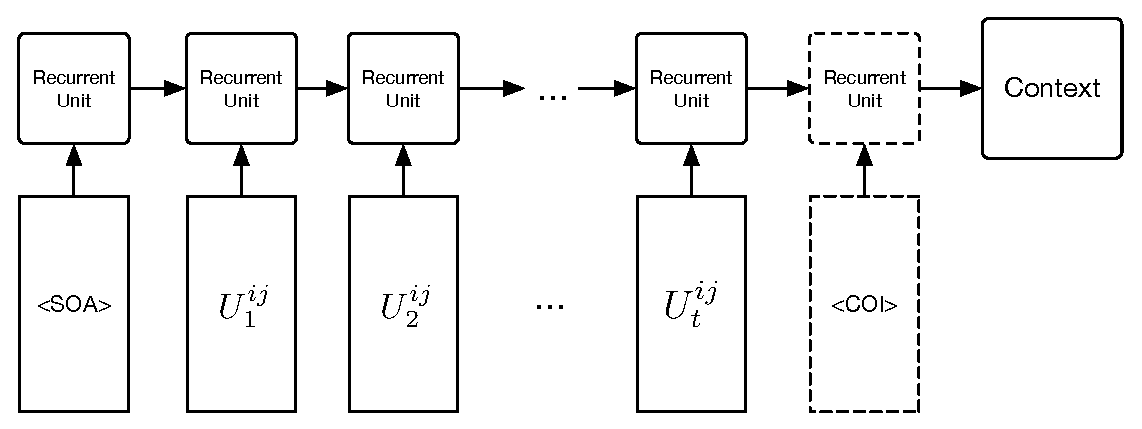
\includegraphics[width=0.7\textwidth]{figures/encoder}
    \caption{An unrolled illustration of context encoder of Action Path Model. 
    In the encoder, 
    a starting mark ``<SOA>'' is used as a sign of start feeding URLs, 
    and a trigger mark ``<COI>'' as
    a sign to trigger decoder to decodes encoded context tensor.
    The trigger mark is automatically inserted after the $k$-th URL while training in the end
    of encoder model over time, $k$ is increasing over time.
    In addition, the recurrent unit is not detailly describeed in the figure but afterwards.}
    \label{fig:encoder}
\end{figure}

Note that the input URLs to encoder recurrent unit are preprocessed through 
url2vec embeddings, which has learned and updated from one-hot encoded vectors to 
densely distributed vectors.

\subsubsection{Context Decoder}

\emph{Context decoder} decodes the context tensor produced by encoder into series of URLs. 
We practically feed a prediction mark ``<SOP>'' (\emph{Start of Prediction}) as a sign 
to initiate the decoding of encoded context. 
In the end of decoder, decoder produces an ending mark ``<EOA>'' (\emph{End of Action}) 
that terminates the decoding process.

Note that the decoder model in training phase and prediction phase is different.
In the training phase, teacher forcing strategy \cite{williams1989learning} is used, 
the strategy supplys observed user actions as inputs in decoder.
In the evaluation phase, decoder uses the output from recurrent unit as input, shown through 
dashed lines in Figure \ref{fig:decoder}.

\begin{figure}
    \centering
    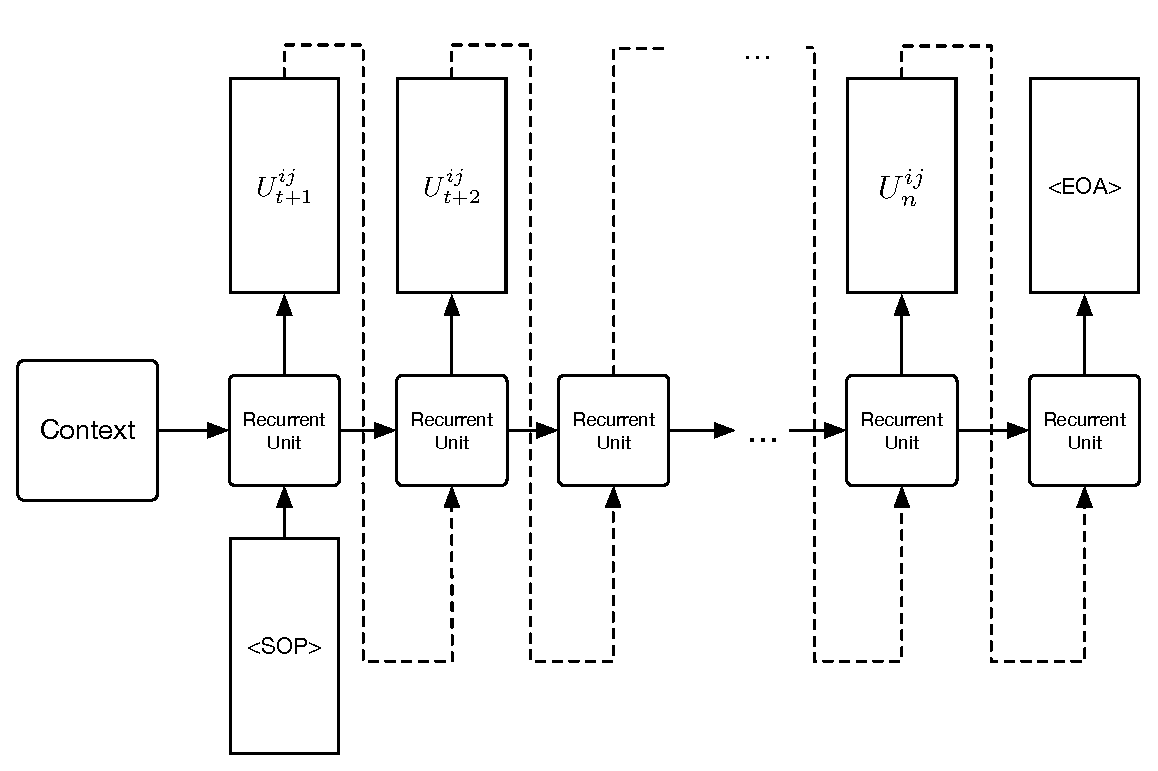
\includegraphics[width=0.7\textwidth]{figures/decoder}
    \caption{Context decoder of Action Path Model. In the decoder, 
    a prediction mark ``<SOP>'' is used to initiate decoding process, 
    and an ending mark ``<EOA>'' as a sign to terminate decode process.
    The output of decoder uses a softmax intermediate operation to magnify and normalize
    the probability of predicted URL embedding.
    In addition, the recurrent unit is not detailly describeed in the figure but afterwards.}
    \label{fig:decoder}
\end{figure}

In our model, a decoder outputs vectors first, and we have two strategy in translating vectors to URLs. 
The first strategy is to use argmax function to select the component with maximum 
probability of a vector, we use this strategy for performance evaluation in 
Section \ref{sec:eval-optimal}. Another strategy is to select
a series of URLs that gains highest joint probability, 
we discusse and use this strategy for action path optimization in Section \ref{sec:optimization}.

\subsubsection{Recurrent Unit}
\label{sec:recurrent-unit}

\textbf{The recurrent unit in the Action Path model is not as standard as original 
LSTM or GRU}, which is one of the major contributions of the thesis. 
In our recurrent unit, when using LSTM as recurrent unit base, we also 
feed time duration $(d^{ij}_1, d^{ij}_2, ..., d^{ij}_n)$
into input gate $I_t$, and others (forget gate $F_t$, output gate $O_t$, 
memory cell $C_t$ and hidden state $h_t$) remains the same:

\begin{align}
\label{eqn:lstm}
\begin{split}
    I_t =& \sigma ( P^{(I)} U^{ij}_t + Q^{(I)} h_{t-1} + \frac{d^{ij}_t}{d^{ij}_t + 1}) ) \\
    F_t =& \sigma ( P^{(F)} U^{ij}_t + Q^{(F)} h_{t-1} + b^{(F)}) \\
    O_t =& \sigma ( P^{(O)} U^{ij}_t + Q^{(O)} h_{t-1} ) \\
    C_t =& F^{(t)} \circ C_{t-1} + I_t \circ \tanh (P^{(C)} U^{ij}_t + Q^{(C)} h_{t-1}) \\
    h_t =& O_t \circ \tanh (C_t)
\end{split}
\end{align}

where $t = 1, 2, ..., n; P^{(I)}, Q^{(I)}, P^{(F)}, Q^{(F)}, P^{(O)}, Q^{(O)}$ are shared weight parameters, 
$b^{(F)}$ is a bias in forget gate $F_t$,
$\circ$ represents element-wise product of two matrices.

When using GRU as recurrent unit base, we feed time duration $(d^{ij}_1, d^{ij}_2, ..., d^{ij}_n)$
in to update gate $Z_t$, and others (reset gate $R_t$, hidden state $h_t$) stay the same:

\begin{align}
\label{eqn:gru}
\begin{split}
    Z_t =& \sigma ( P^{(Z)} U^{ij}_t + Q^{(Z)} h_{t-1} + \frac{d^{ij}_t}{d^{ij}_t + 1} ) \\
    R_t =& \sigma ( P^{(R)} U^{ij}_t + Q^{(R)} h_{t-1} ) \\
    h_t =& ( 1 - Z_t ) \circ \tanh ( P^{(H)} U^{ij}_t + Q^{(H)} h_{t-1} ) + Z_t \circ h_{t-1}
\end{split}
\end{align}

where $t = 1, 2, ..., n; P^{(Z)}, Q^{(Z)}, P^{(R)}, Q^{(R)}, P^{(H)}, Q^{(H)}$ are shared weight parameters, 
$\circ$ represents element-wise product of two matrices.

\paragraph{Remark 1} The units we described in this section is neither LSTM nor GRU since
the input gate $I_t$ or update gate $Z_t$ introduces time duration $d^{ij}_t$ as input,
which is different than a simple constant bias in the original learnable bias in these gates. 
It is worth mentioning that adding bias to the gates are helpful to 
improve learning performance in LSTM \cite{Jozefowicz:2015:EER:3045118.3045367}, 
we also use the trick in our model as shown in $F_t$ of Equation \ref{eqn:lstm}.

\paragraph{Remark 2} The term $\frac{d^{ij}_t}{d^{ij}_t + 1}$ is a squashing mechanism,
it normalizes $d^{ij}_t$ from $(0, \infty)$ to $(0, 1)$.

\subsubsection{Ending Mark Interpretation}
\label{sec:mark-interpretation}

In context decoder, we mentioned an ending mark ``<EOA>'' that indicates the termination 
decoding process. However, the ending mark is different than other marks, since in practice,
``<EOA>'' is represented in different symbols of behavior-based categorical clickstream, which as a label to
involve classification of user actions.

Assume action paths are labeled by one-hot encoded ending marks 
$\text{EOA}_1, \text{EOA}_2, ..., \text{EOA}_m$ and the last output
of decoder hidden state is $h_n$, we have:

\begin{align}
\label{eqn:mark}
\begin{split}
    \hat{y} =& \text{argmax} (\text{softmax} (W^{(M)} h_n)) \\
    \hat{y} \in& \{ \text{EOA}_1, \text{EOA}_2, ..., \text{EOA}_m \}
\end{split}
\end{align}

where $W^{(M)}$ is a weight parameter, and $m$ is the number of ending mark categories.

\subsection{Action Path Optimization}
\label{sec:optimization}

In traditional classification models, the arguments of the maxima (argmax) is used to select
labels with highest probability, scilicet, argmax selects predicted URLs with highest probability
of user action from decoder outputs. However, this method is under the condition of all outputs
are independent in probability, which is not suitable to our action path optimization senario.

In previous sections, our model feeds an input clickstream $(U^{ij}_1, U^{ij}_2, ..., U^{ij}_t)$,
and produce an output $(o_1, o_2, ..., o_{m})$ that expect close to actual clickstream 
$(U^{ij}_{t+1}, U^{ij}_{t+2}, ..., U^{ij}_n)$.
Then the probability of expected clickstream is a conditional probability under 
the input clickstream, i.e. we need to solve an optimization problem:

\begin{align}
\label{eqn:optimize}
\begin{split}
    & \operatorname*{argmax}_{o} p( o_1, o_2, ..., o_{m} | U^{ij}_1, U^{ij}_2, ..., U^{ij}_t ) \\
   =& \operatorname*{argmax}_{o} \prod_{k=1}^{m} p(o_{k} | U^{ij}_1, ..., U^{ij}_t, o_1, ..., o_{k-1}) \\
   =& \operatorname*{argmax}_{o} \sum_{k=1}^{m} \log p(o_{k} | U^{ij}_1, ..., U^{ij}_t, o_1, ..., o_{k-1})
\end{split}
\end{align}

A heuristic approach can solve the optimization problem efficiently, namely beam search 
\cite{DBLP:journals/corr/abs-1211-3711}.
In each step of decoder output, we reserve the top-$k$ best combinations of URLs and 
eliminate the rest of URLs from evaluation, and finally selects $k$ best clickstreams.
The pseudocode is given that adapts vanilla beam search to URL prediction search 
in Algorithm \ref{algo:optimize}.

~\\

\begin{algorithm}[H]
\label{algo:optimize}
\SetAlgoLined
\SetKwInOut{Input}{input}\SetKwInOut{Output}{output}
\Input{Decoder outputs $(o_1, o_2, ..., o_{m})$,\\
        Number of candidates $k$}
\Output{k clickstream candidates with highest probability}
\Begin{
    Initialize empty $\text{clickstreams}$ list \\
    \For{$o$ $\in$ $(o_1, o_2, ..., o_{m})$}{
        Initialize empty $candidates$ list \\
        \For{$\text{clickstream}$ $\in$ $\text{clickstreams}$}{
            \For{page $\in$ $o$)}{
                candidates.append([clickstream.append(page), $log(p(\text{clickstream})) + log(p(\text{page}))$]) \\
            }
        }
        ordered = descending order sort candidates by score \\
        clickstreams = ordered[:k]
    }
}
\caption{Output Clickstream Search}
\end{algorithm}

~\\

\paragraph{Remark} The algorithm produces an heuristic output 
with given clickstream context. Combining with \emph{url2vec} model, the prediction
can heuristically optimize the click path of a specific user since the embeddings are trained 
over all possible action path. For instance, a distraction advertisement page will not appear
after optimization because the embedding of advertisement page is far from a desired page
if embeddings are learned correctly.

% This chapter proposed several models that characterized a method to modeling user actions
% on the Web.

\cleardoublepage